% Graphic for TeX using PGF
% Title: C:\Users\Nicolas Chicaiza\Sourcetree\Metodología de la Investigación\Enfoque Marco Lógico\Esquemas\Árbol de Participación\arbolParticipacion.dia
% Creator: Dia v0.97.2
% CreationDate: Mon May 03 00:48:48 2021
% For: Nicolas Chicaiza
% \usepackage{tikz}
% The following commands are not supported in PSTricks at present
% We define them conditionally, so when they are implemented,
% this pgf file will use them.
\ifx\du\undefined
  \newlength{\du}
\fi
\setlength{\du}{15\unitlength}
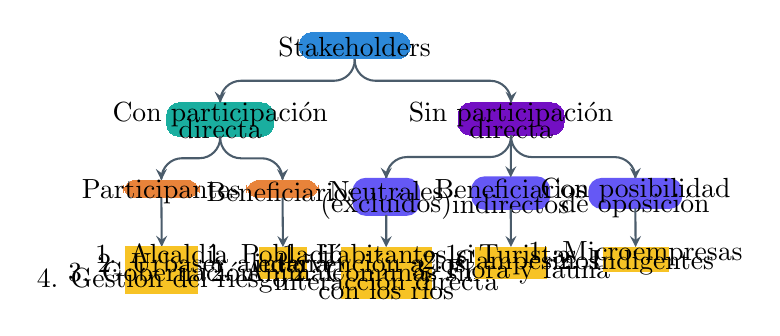
\begin{tikzpicture}
\pgftransformxscale{1.000000}
\pgftransformyscale{-1.000000}
\definecolor{dialinecolor}{rgb}{0.000000, 0.000000, 0.000000}
\pgfsetstrokecolor{dialinecolor}
\definecolor{dialinecolor}{rgb}{1.000000, 1.000000, 1.000000}
\pgfsetfillcolor{dialinecolor}
\pgfsetlinewidth{0.000000\du}
\pgfsetdash{}{0pt}
\pgfsetdash{}{0pt}
\pgfsetroundjoin
{\pgfsetcornersarced{\pgfpoint{0.300000\du}{0.300000\du}}\definecolor{dialinecolor}{rgb}{0.172549, 0.533333, 0.850980}
\pgfsetfillcolor{dialinecolor}
\fill (49.907800\du,8.337130\du)--(49.907800\du,8.970333\du)--(52.579713\du,8.970333\du)--(52.579713\du,8.337130\du)--cycle;
}{\pgfsetcornersarced{\pgfpoint{0.300000\du}{0.300000\du}}\definecolor{dialinecolor}{rgb}{0.172549, 0.533333, 0.850980}
\pgfsetstrokecolor{dialinecolor}
\draw (49.907800\du,8.337130\du)--(49.907800\du,8.970333\du)--(52.579713\du,8.970333\du)--(52.579713\du,8.337130\du)--cycle;
}% setfont left to latex
\definecolor{dialinecolor}{rgb}{1.000000, 1.000000, 1.000000}
\pgfsetstrokecolor{dialinecolor}
\node at (51.243756\du,8.674630\du){Stakeholders};
\pgfsetlinewidth{0.000000\du}
\pgfsetdash{}{0pt}
\pgfsetdash{}{0pt}
\pgfsetroundjoin
{\pgfsetcornersarced{\pgfpoint{0.300000\du}{0.300000\du}}\definecolor{dialinecolor}{rgb}{0.450980, 0.058824, 0.764706}
\pgfsetfillcolor{dialinecolor}
\fill (53.735000\du,10.029400\du)--(53.735000\du,10.812075\du)--(56.285803\du,10.812075\du)--(56.285803\du,10.029400\du)--cycle;
}{\pgfsetcornersarced{\pgfpoint{0.300000\du}{0.300000\du}}\definecolor{dialinecolor}{rgb}{0.450980, 0.058824, 0.764706}
\pgfsetstrokecolor{dialinecolor}
\draw (53.735000\du,10.029400\du)--(53.735000\du,10.812075\du)--(56.285803\du,10.812075\du)--(56.285803\du,10.029400\du)--cycle;
}\pgfsetlinewidth{0.050000\du}
\pgfsetdash{}{0pt}
\pgfsetdash{}{0pt}
\pgfsetroundjoin
\pgfsetbuttcap
{
\definecolor{dialinecolor}{rgb}{0.294118, 0.360784, 0.419608}
\pgfsetfillcolor{dialinecolor}
% was here!!!
\pgfsetarrowsend{stealth}
{\pgfsetcornersarced{\pgfpoint{0.500000\du}{0.500000\du}}\definecolor{dialinecolor}{rgb}{0.294118, 0.360784, 0.419608}
\pgfsetstrokecolor{dialinecolor}
\draw (51.243756\du,8.970333\du)--(51.243756\du,9.499866\du)--(55.010402\du,9.499866\du)--(55.010402\du,10.029400\du);
}}
% setfont left to latex
\definecolor{dialinecolor}{rgb}{1.000000, 1.000000, 1.000000}
\pgfsetstrokecolor{dialinecolor}
\node at (55.010402\du,10.311900\du){Sin participación};
% setfont left to latex
\definecolor{dialinecolor}{rgb}{1.000000, 1.000000, 1.000000}
\pgfsetstrokecolor{dialinecolor}
\node at (55.010402\du,10.664678\du){directa};
\pgfsetlinewidth{0.000000\du}
\pgfsetdash{}{0pt}
\pgfsetdash{}{0pt}
\pgfsetroundjoin
{\pgfsetcornersarced{\pgfpoint{0.300000\du}{0.300000\du}}\definecolor{dialinecolor}{rgb}{0.101961, 0.682353, 0.623529}
\pgfsetfillcolor{dialinecolor}
\fill (46.713200\du,10.029400\du)--(46.713200\du,10.839596\du)--(49.293356\du,10.839596\du)--(49.293356\du,10.029400\du)--cycle;
}{\pgfsetcornersarced{\pgfpoint{0.300000\du}{0.300000\du}}\definecolor{dialinecolor}{rgb}{0.101961, 0.682353, 0.623529}
\pgfsetstrokecolor{dialinecolor}
\draw (46.713200\du,10.029400\du)--(46.713200\du,10.839596\du)--(49.293356\du,10.839596\du)--(49.293356\du,10.029400\du)--cycle;
}% setfont left to latex
\definecolor{dialinecolor}{rgb}{1.000000, 1.000000, 1.000000}
\pgfsetstrokecolor{dialinecolor}
\node at (48.003278\du,10.311900\du){Con participación};
% setfont left to latex
\definecolor{dialinecolor}{rgb}{1.000000, 1.000000, 1.000000}
\pgfsetstrokecolor{dialinecolor}
\node at (48.003278\du,10.664678\du){directa};
\pgfsetlinewidth{0.050000\du}
\pgfsetdash{}{0pt}
\pgfsetdash{}{0pt}
\pgfsetroundjoin
\pgfsetbuttcap
{
\definecolor{dialinecolor}{rgb}{0.294118, 0.360784, 0.419608}
\pgfsetfillcolor{dialinecolor}
% was here!!!
\pgfsetarrowsend{stealth}
{\pgfsetcornersarced{\pgfpoint{0.500000\du}{0.500000\du}}\definecolor{dialinecolor}{rgb}{0.294118, 0.360784, 0.419608}
\pgfsetstrokecolor{dialinecolor}
\draw (51.243756\du,8.970333\du)--(51.243756\du,9.499866\du)--(48.003278\du,9.499866\du)--(48.003278\du,10.029400\du);
}}
\pgfsetlinewidth{0.050000\du}
\pgfsetdash{}{0pt}
\pgfsetdash{}{0pt}
\pgfsetroundjoin
\pgfsetbuttcap
{
\definecolor{dialinecolor}{rgb}{0.294118, 0.360784, 0.419608}
\pgfsetfillcolor{dialinecolor}
% was here!!!
\pgfsetarrowsend{stealth}
{\pgfsetcornersarced{\pgfpoint{0.500000\du}{0.500000\du}}\definecolor{dialinecolor}{rgb}{0.294118, 0.360784, 0.419608}
\pgfsetstrokecolor{dialinecolor}
\draw (48.003278\du,10.839596\du)--(48.003278\du,11.367398\du)--(49.505825\du,11.367398\du)--(49.505825\du,11.895200\du);
}}
\pgfsetlinewidth{0.050000\du}
\pgfsetdash{}{0pt}
\pgfsetdash{}{0pt}
\pgfsetroundjoin
\pgfsetbuttcap
{
\definecolor{dialinecolor}{rgb}{0.294118, 0.360784, 0.419608}
\pgfsetfillcolor{dialinecolor}
% was here!!!
\pgfsetarrowsend{stealth}
{\pgfsetcornersarced{\pgfpoint{0.500000\du}{0.500000\du}}\definecolor{dialinecolor}{rgb}{0.294118, 0.360784, 0.419608}
\pgfsetstrokecolor{dialinecolor}
\draw (48.003278\du,10.839596\du)--(48.003278\du,11.365548\du)--(46.586887\du,11.365548\du)--(46.586887\du,11.891500\du);
}}
\pgfsetlinewidth{0.000000\du}
\pgfsetdash{}{0pt}
\pgfsetdash{}{0pt}
\pgfsetroundjoin
{\pgfsetcornersarced{\pgfpoint{0.300000\du}{0.300000\du}}\definecolor{dialinecolor}{rgb}{0.909804, 0.513726, 0.227451}
\pgfsetfillcolor{dialinecolor}
\fill (45.677300\du,11.891500\du)--(45.677300\du,12.318853\du)--(47.496475\du,12.318853\du)--(47.496475\du,11.891500\du)--cycle;
}{\pgfsetcornersarced{\pgfpoint{0.300000\du}{0.300000\du}}\definecolor{dialinecolor}{rgb}{0.909804, 0.513726, 0.227451}
\pgfsetstrokecolor{dialinecolor}
\draw (45.677300\du,11.891500\du)--(45.677300\du,12.318853\du)--(47.496475\du,12.318853\du)--(47.496475\du,11.891500\du)--cycle;
}\pgfsetlinewidth{0.000000\du}
\pgfsetdash{}{0pt}
\pgfsetdash{}{0pt}
\pgfsetroundjoin
{\pgfsetcornersarced{\pgfpoint{0.300000\du}{0.300000\du}}\definecolor{dialinecolor}{rgb}{0.909804, 0.513726, 0.227451}
\pgfsetfillcolor{dialinecolor}
\fill (48.639800\du,11.895200\du)--(48.639800\du,12.312653\du)--(50.371850\du,12.312653\du)--(50.371850\du,11.895200\du)--cycle;
}{\pgfsetcornersarced{\pgfpoint{0.300000\du}{0.300000\du}}\definecolor{dialinecolor}{rgb}{0.909804, 0.513726, 0.227451}
\pgfsetstrokecolor{dialinecolor}
\draw (48.639800\du,11.895200\du)--(48.639800\du,12.312653\du)--(50.371850\du,12.312653\du)--(50.371850\du,11.895200\du)--cycle;
}% setfont left to latex
\definecolor{dialinecolor}{rgb}{1.000000, 1.000000, 1.000000}
\pgfsetstrokecolor{dialinecolor}
\node at (46.586887\du,12.174000\du){Participantes};
% setfont left to latex
\definecolor{dialinecolor}{rgb}{1.000000, 1.000000, 1.000000}
\pgfsetstrokecolor{dialinecolor}
\node at (49.505825\du,12.177700\du){Beneficiarios};
\pgfsetlinewidth{0.050000\du}
\pgfsetdash{}{0pt}
\pgfsetdash{}{0pt}
\pgfsetroundjoin
\pgfsetbuttcap
{
\definecolor{dialinecolor}{rgb}{0.294118, 0.360784, 0.419608}
\pgfsetfillcolor{dialinecolor}
% was here!!!
\pgfsetarrowsend{stealth}
{\pgfsetcornersarced{\pgfpoint{0.500000\du}{0.500000\du}}\definecolor{dialinecolor}{rgb}{0.294118, 0.360784, 0.419608}
\pgfsetstrokecolor{dialinecolor}
\draw (55.010402\du,10.812075\du)--(55.010402\du,11.338351\du)--(58.005318\du,11.338351\du)--(58.005318\du,11.864628\du);
}}
\pgfsetlinewidth{0.050000\du}
\pgfsetdash{}{0pt}
\pgfsetdash{}{0pt}
\pgfsetroundjoin
\pgfsetbuttcap
{
\definecolor{dialinecolor}{rgb}{0.294118, 0.360784, 0.419608}
\pgfsetfillcolor{dialinecolor}
% was here!!!
\pgfsetarrowsend{stealth}
{\pgfsetcornersarced{\pgfpoint{0.500000\du}{0.500000\du}}\definecolor{dialinecolor}{rgb}{0.294118, 0.360784, 0.419608}
\pgfsetstrokecolor{dialinecolor}
\draw (55.010402\du,10.812075\du)--(55.010402\du,11.337101\du)--(52.003848\du,11.337101\du)--(52.003848\du,11.862128\du);
}}
\pgfsetlinewidth{0.050000\du}
\pgfsetdash{}{0pt}
\pgfsetdash{}{0pt}
\pgfsetroundjoin
{\pgfsetcornersarced{\pgfpoint{0.300000\du}{0.300000\du}}\definecolor{dialinecolor}{rgb}{0.396078, 0.345098, 0.960784}
\pgfsetfillcolor{dialinecolor}
\fill (51.214800\du,11.862128\du)--(51.214800\du,12.728786\du)--(52.792896\du,12.728786\du)--(52.792896\du,11.862128\du)--cycle;
}{\pgfsetcornersarced{\pgfpoint{0.300000\du}{0.300000\du}}\definecolor{dialinecolor}{rgb}{0.396078, 0.345098, 0.960784}
\pgfsetstrokecolor{dialinecolor}
\draw (51.214800\du,11.862128\du)--(51.214800\du,12.728786\du)--(52.792896\du,12.728786\du)--(52.792896\du,11.862128\du)--cycle;
}\pgfsetlinewidth{0.050000\du}
\pgfsetdash{}{0pt}
\pgfsetdash{}{0pt}
\pgfsetroundjoin
{\pgfsetcornersarced{\pgfpoint{0.300000\du}{0.300000\du}}\definecolor{dialinecolor}{rgb}{0.396078, 0.345098, 0.960784}
\pgfsetfillcolor{dialinecolor}
\fill (56.896000\du,11.864628\du)--(56.896000\du,12.563877\du)--(59.114637\du,12.563877\du)--(59.114637\du,11.864628\du)--cycle;
}{\pgfsetcornersarced{\pgfpoint{0.300000\du}{0.300000\du}}\definecolor{dialinecolor}{rgb}{0.396078, 0.345098, 0.960784}
\pgfsetstrokecolor{dialinecolor}
\draw (56.896000\du,11.864628\du)--(56.896000\du,12.563877\du)--(59.114637\du,12.563877\du)--(59.114637\du,11.864628\du)--cycle;
}\pgfsetlinewidth{0.050000\du}
\pgfsetdash{}{0pt}
\pgfsetdash{}{0pt}
\pgfsetroundjoin
{\pgfsetcornersarced{\pgfpoint{0.300000\du}{0.300000\du}}\definecolor{dialinecolor}{rgb}{0.396078, 0.345098, 0.960784}
\pgfsetfillcolor{dialinecolor}
\fill (54.077300\du,11.826800\du)--(54.077300\du,12.582545\du)--(55.926869\du,12.582545\du)--(55.926869\du,11.826800\du)--cycle;
}{\pgfsetcornersarced{\pgfpoint{0.300000\du}{0.300000\du}}\definecolor{dialinecolor}{rgb}{0.396078, 0.345098, 0.960784}
\pgfsetstrokecolor{dialinecolor}
\draw (54.077300\du,11.826800\du)--(54.077300\du,12.582545\du)--(55.926869\du,12.582545\du)--(55.926869\du,11.826800\du)--cycle;
}\pgfsetlinewidth{0.050000\du}
\pgfsetdash{}{0pt}
\pgfsetdash{}{0pt}
\pgfsetbuttcap
{
\definecolor{dialinecolor}{rgb}{0.294118, 0.360784, 0.419608}
\pgfsetfillcolor{dialinecolor}
% was here!!!
\pgfsetarrowsend{stealth}
\definecolor{dialinecolor}{rgb}{0.294118, 0.360784, 0.419608}
\pgfsetstrokecolor{dialinecolor}
\draw (55.010402\du,10.812075\du)--(55.002085\du,11.826800\du);
}
% setfont left to latex
\definecolor{dialinecolor}{rgb}{1.000000, 1.000000, 1.000000}
\pgfsetstrokecolor{dialinecolor}
\node at (52.003848\du,12.144628\du){Neutrales};
% setfont left to latex
\definecolor{dialinecolor}{rgb}{1.000000, 1.000000, 1.000000}
\pgfsetstrokecolor{dialinecolor}
\node at (52.003848\du,12.497405\du){(excluídos)};
% setfont left to latex
\definecolor{dialinecolor}{rgb}{1.000000, 1.000000, 1.000000}
\pgfsetstrokecolor{dialinecolor}
\node at (55.002085\du,12.109300\du){Beneficiarios};
% setfont left to latex
\definecolor{dialinecolor}{rgb}{1.000000, 1.000000, 1.000000}
\pgfsetstrokecolor{dialinecolor}
\node at (55.002085\du,12.462078\du){indirectos};
% setfont left to latex
\definecolor{dialinecolor}{rgb}{1.000000, 1.000000, 1.000000}
\pgfsetstrokecolor{dialinecolor}
\node at (58.005318\du,12.147128\du){Con posibilidad};
% setfont left to latex
\definecolor{dialinecolor}{rgb}{1.000000, 1.000000, 1.000000}
\pgfsetstrokecolor{dialinecolor}
\node at (58.005318\du,12.499905\du){ de oposición};
\pgfsetlinewidth{0.050000\du}
\pgfsetdash{}{0pt}
\pgfsetdash{}{0pt}
\pgfsetbuttcap
{
\definecolor{dialinecolor}{rgb}{0.294118, 0.360784, 0.419608}
\pgfsetfillcolor{dialinecolor}
% was here!!!
\pgfsetarrowsend{stealth}
\definecolor{dialinecolor}{rgb}{0.294118, 0.360784, 0.419608}
\pgfsetstrokecolor{dialinecolor}
\draw (46.586887\du,12.318853\du)--(46.595303\du,13.500100\du);
}
\pgfsetlinewidth{0.000000\du}
\pgfsetdash{}{0pt}
\pgfsetdash{}{0pt}
\pgfsetmiterjoin
\definecolor{dialinecolor}{rgb}{0.968627, 0.764706, 0.145098}
\pgfsetfillcolor{dialinecolor}
\fill (45.727300\du,13.500100\du)--(45.727300\du,14.616879\du)--(47.463306\du,14.616879\du)--(47.463306\du,13.500100\du)--cycle;
\definecolor{dialinecolor}{rgb}{0.968627, 0.764706, 0.145098}
\pgfsetstrokecolor{dialinecolor}
\draw (45.727300\du,13.500100\du)--(45.727300\du,14.616879\du)--(47.463306\du,14.616879\du)--(47.463306\du,13.500100\du)--cycle;
% setfont left to latex
\definecolor{dialinecolor}{rgb}{0.176471, 0.231373, 0.270588}
\pgfsetstrokecolor{dialinecolor}
\node at (46.595303\du,13.670100\du){1. Alcaldía};
% setfont left to latex
\definecolor{dialinecolor}{rgb}{0.176471, 0.231373, 0.270588}
\pgfsetstrokecolor{dialinecolor}
\node at (46.595303\du,13.881767\du){2. Urbaser};
% setfont left to latex
\definecolor{dialinecolor}{rgb}{0.176471, 0.231373, 0.270588}
\pgfsetstrokecolor{dialinecolor}
\node at (46.595303\du,14.093433\du){3. Gobernación};
% setfont left to latex
\definecolor{dialinecolor}{rgb}{0.176471, 0.231373, 0.270588}
\pgfsetstrokecolor{dialinecolor}
\node at (46.595303\du,14.305100\du){4. Gestión del riesgo};
\pgfsetlinewidth{0.050000\du}
\pgfsetdash{}{0pt}
\pgfsetdash{}{0pt}
\pgfsetbuttcap
{
\definecolor{dialinecolor}{rgb}{0.294118, 0.360784, 0.419608}
\pgfsetfillcolor{dialinecolor}
% was here!!!
\pgfsetarrowsend{stealth}
\definecolor{dialinecolor}{rgb}{0.294118, 0.360784, 0.419608}
\pgfsetstrokecolor{dialinecolor}
\draw (49.505825\du,12.312653\du)--(49.515073\du,13.506400\du);
}
\pgfsetlinewidth{0.000000\du}
\pgfsetdash{}{0pt}
\pgfsetdash{}{0pt}
\pgfsetmiterjoin
\definecolor{dialinecolor}{rgb}{0.968627, 0.764706, 0.145098}
\pgfsetfillcolor{dialinecolor}
\fill (48.939800\du,13.506400\du)--(48.939800\du,14.263161\du)--(50.090347\du,14.263161\du)--(50.090347\du,13.506400\du)--cycle;
\definecolor{dialinecolor}{rgb}{0.968627, 0.764706, 0.145098}
\pgfsetstrokecolor{dialinecolor}
\draw (48.939800\du,13.506400\du)--(48.939800\du,14.263161\du)--(50.090347\du,14.263161\du)--(50.090347\du,13.506400\du)--cycle;
% setfont left to latex
\definecolor{dialinecolor}{rgb}{0.176471, 0.231373, 0.270588}
\pgfsetstrokecolor{dialinecolor}
\node at (49.515073\du,13.676400\du){1. Población};
% setfont left to latex
\definecolor{dialinecolor}{rgb}{0.176471, 0.231373, 0.270588}
\pgfsetstrokecolor{dialinecolor}
\node at (49.515073\du,13.888067\du){aledaña};
% setfont left to latex
\definecolor{dialinecolor}{rgb}{0.176471, 0.231373, 0.270588}
\pgfsetstrokecolor{dialinecolor}
\node at (49.515073\du,14.099733\du){2. Animales};
\pgfsetlinewidth{0.050000\du}
\pgfsetdash{}{0pt}
\pgfsetdash{}{0pt}
\pgfsetbuttcap
{
\definecolor{dialinecolor}{rgb}{0.294118, 0.360784, 0.419608}
\pgfsetfillcolor{dialinecolor}
% was here!!!
\pgfsetarrowsend{stealth}
\definecolor{dialinecolor}{rgb}{0.294118, 0.360784, 0.419608}
\pgfsetstrokecolor{dialinecolor}
\draw (52.003848\du,12.728786\du)--(52.002368\du,13.509200\du);
}
\pgfsetlinewidth{0.000000\du}
\pgfsetdash{}{0pt}
\pgfsetdash{}{0pt}
\pgfsetmiterjoin
\definecolor{dialinecolor}{rgb}{0.968627, 0.764706, 0.145098}
\pgfsetfillcolor{dialinecolor}
\fill (50.918000\du,13.509200\du)--(50.918000\du,14.741530\du)--(53.086735\du,14.741530\du)--(53.086735\du,13.509200\du)--cycle;
\definecolor{dialinecolor}{rgb}{0.968627, 0.764706, 0.145098}
\pgfsetstrokecolor{dialinecolor}
\draw (50.918000\du,13.509200\du)--(50.918000\du,14.741530\du)--(53.086735\du,14.741530\du)--(53.086735\du,13.509200\du)--cycle;
% setfont left to latex
\definecolor{dialinecolor}{rgb}{0.176471, 0.231373, 0.270588}
\pgfsetstrokecolor{dialinecolor}
\node at (52.002368\du,13.679200\du){1. Habitantes sin};
% setfont left to latex
\definecolor{dialinecolor}{rgb}{0.176471, 0.231373, 0.270588}
\pgfsetstrokecolor{dialinecolor}
\node at (52.002368\du,13.890867\du){intervención a los ríos};
% setfont left to latex
\definecolor{dialinecolor}{rgb}{0.176471, 0.231373, 0.270588}
\pgfsetstrokecolor{dialinecolor}
\node at (52.002368\du,14.102533\du){2. Comunas sin };
% setfont left to latex
\definecolor{dialinecolor}{rgb}{0.176471, 0.231373, 0.270588}
\pgfsetstrokecolor{dialinecolor}
\node at (52.002368\du,14.314200\du){interacción directa };
% setfont left to latex
\definecolor{dialinecolor}{rgb}{0.176471, 0.231373, 0.270588}
\pgfsetstrokecolor{dialinecolor}
\node at (52.002368\du,14.525867\du){con los ríos};
\pgfsetlinewidth{0.050000\du}
\pgfsetdash{}{0pt}
\pgfsetdash{}{0pt}
\pgfsetbuttcap
{
\definecolor{dialinecolor}{rgb}{0.294118, 0.360784, 0.419608}
\pgfsetfillcolor{dialinecolor}
% was here!!!
\pgfsetarrowsend{stealth}
\definecolor{dialinecolor}{rgb}{0.294118, 0.360784, 0.419608}
\pgfsetstrokecolor{dialinecolor}
\draw (55.002085\du,12.582545\du)--(55.008271\du,13.504800\du);
}
\pgfsetlinewidth{0.000000\du}
\pgfsetdash{}{0pt}
\pgfsetdash{}{0pt}
\pgfsetmiterjoin
\definecolor{dialinecolor}{rgb}{0.968627, 0.764706, 0.145098}
\pgfsetfillcolor{dialinecolor}
\fill (54.161100\du,13.504800\du)--(54.161100\du,14.268839\du)--(55.855443\du,14.268839\du)--(55.855443\du,13.504800\du)--cycle;
\definecolor{dialinecolor}{rgb}{0.968627, 0.764706, 0.145098}
\pgfsetstrokecolor{dialinecolor}
\draw (54.161100\du,13.504800\du)--(54.161100\du,14.268839\du)--(55.855443\du,14.268839\du)--(55.855443\du,13.504800\du)--cycle;
% setfont left to latex
\definecolor{dialinecolor}{rgb}{0.176471, 0.231373, 0.270588}
\pgfsetstrokecolor{dialinecolor}
\node at (55.008271\du,13.674800\du){1. Turistas};
% setfont left to latex
\definecolor{dialinecolor}{rgb}{0.176471, 0.231373, 0.270588}
\pgfsetstrokecolor{dialinecolor}
\node at (55.008271\du,13.886467\du){2. Campesinos};
% setfont left to latex
\definecolor{dialinecolor}{rgb}{0.176471, 0.231373, 0.270588}
\pgfsetstrokecolor{dialinecolor}
\node at (55.008271\du,14.098133\du){3. Flora y fauna};
\pgfsetlinewidth{0.050000\du}
\pgfsetdash{}{0pt}
\pgfsetdash{}{0pt}
\pgfsetbuttcap
{
\definecolor{dialinecolor}{rgb}{0.294118, 0.360784, 0.419608}
\pgfsetfillcolor{dialinecolor}
% was here!!!
\pgfsetarrowsend{stealth}
\definecolor{dialinecolor}{rgb}{0.294118, 0.360784, 0.419608}
\pgfsetstrokecolor{dialinecolor}
\draw (58.005318\du,12.563877\du)--(58.010248\du,13.506400\du);
}
\pgfsetlinewidth{0.000000\du}
\pgfsetdash{}{0pt}
\pgfsetdash{}{0pt}
\pgfsetmiterjoin
\definecolor{dialinecolor}{rgb}{0.968627, 0.764706, 0.145098}
\pgfsetfillcolor{dialinecolor}
\fill (57.227300\du,13.506400\du)--(57.227300\du,14.087106\du)--(58.793197\du,14.087106\du)--(58.793197\du,13.506400\du)--cycle;
\definecolor{dialinecolor}{rgb}{0.968627, 0.764706, 0.145098}
\pgfsetstrokecolor{dialinecolor}
\draw (57.227300\du,13.506400\du)--(57.227300\du,14.087106\du)--(58.793197\du,14.087106\du)--(58.793197\du,13.506400\du)--cycle;
% setfont left to latex
\definecolor{dialinecolor}{rgb}{0.176471, 0.231373, 0.270588}
\pgfsetstrokecolor{dialinecolor}
\node at (58.010248\du,13.676400\du){1. Microempresas};
% setfont left to latex
\definecolor{dialinecolor}{rgb}{0.176471, 0.231373, 0.270588}
\pgfsetstrokecolor{dialinecolor}
\node at (58.010248\du,13.888067\du){2. Indigentes};
\end{tikzpicture}
